%!TEX root = ../../common/main.tex

\chapter{Conclusion and outlook}
\label{ch:conclusion}

After the first run of the \LHC machine and an efficient data taking period the
foundation of the \SM appears to be solid. The discovery of the Higgs boson
\cite{Aad:2015zhl} endorses the theoretical framework and is a huge success of
the particle physics community. Still, the evidence of \BSM physics is not
deniable. Missing observations of \BSM effects like the observation of heavy
super-symmetric particles or a suitable dark matter candidate dash the hope of
new findings at the \si{TeV}-scale. \RunTwo of the \LHC at nearly the design
centre-of-mass energy of $\SI{13}{TeV}$ will be crucial for the future of the
particle physics community and the design of future experiments.

While direct searches for new heavy particle are constraint by the available
collision energies, indirect searches are sensible to \BSM effects through
higher order contributions. The \LHCb experiment was therefore designed and
built to have the ability to perform high precision tests of the \SM in decays
of \B and \D mesons and to identify possible deviations from the \SM.
Especially, the measurement of \CP violation in the decay of \BdToJpsiKS acts as
a poster child with small theoretical uncertainties, at least one final state
that is easy to reconstruct, and a relatively high event yield.

The measurement of the \CP parameters \SJpsiKS and \CJpsiKS presented in this
thesis was realised on a dataset corresponding to an integrated luminosity of
$\SI{3.0}{\per\femto\barn}$ recorded by the \LHCb experiment in
\acl{protonproton} collisions at centre-of-mass energies of $\num{7}$ and
$\SI{8}{\TeV}$. The sample contains $\num{41500}$ reconstructed $\BdToJpsiKS$
candidates with a flavour tagging decision assigned by either the combination of
the \acl{OS} tagging algorithms or by the \acl{SSpi} tagging algorithm. Using an
\acl{uEML} fit the \CP parameters \SJpsiKS and \CJpsiKS are measured to be
%
\begin{equation*}
  \begin{split}
    \SJpsiKS &= \phantom{-}\num{0.731} \pm \num{0.035} \statp \pm \num{0.020} \systp \eqcm\eqand \\
    \CJpsiKS &=           \num{-0.038} \pm \num{0.032} \statp \pm \num{0.005} \systp \eqcm
  \end{split}
\end{equation*}
%
with a statistical correlation coefficient of $\rho(\SJpsiKS,\CJpsiKS) =
\num{0.483}$. With the parameter \CJpsiKS fixed to zero the measurement yields
$\SJpsiKS = \sintwobeta = \num{0.746 +- 0.030}\statp$.

The measurement improves the previous \LHCb result \cite{Aaij:1497268} by
including a larger dataset, additional trigger lines, an optimised candidate
selection and by incorporating the \SSpi tagger decisions. It is by now the most
precise measurement of \CP violation at a hadron collider and is in excellent
agreement with the current world average. \Cref{fig:conclusion:ckm_fitter_15}
shows the ${(\dquark,\bquark)}$ unitarity triangle in the
${(\ovE{\rho},\ovE{\eta})}$-plane from a global fit incorporating all measured
\CKM parameters \cite{Charles:2004jd} except from the ones reported here that is
additionally shown to allow for a better comparison.
%
\begin{figure}[ht]
\centering
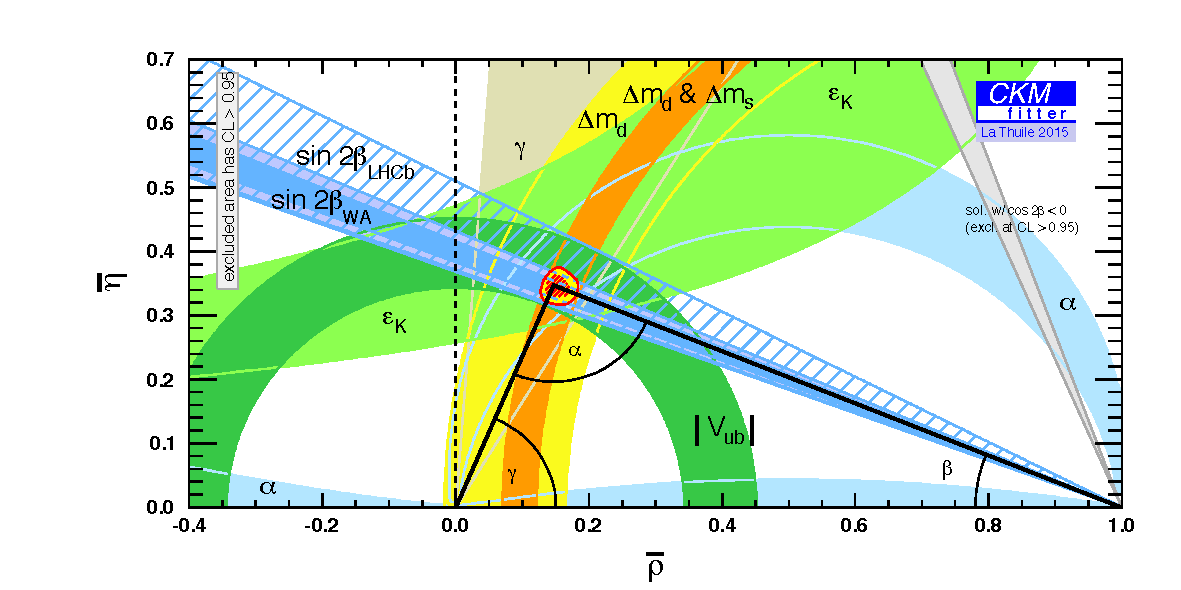
\includegraphics[width=1\textwidth]{private/content/conclusions/figs/ckmfitter_summer15.pdf}
\caption{Constraints on the ${(\dquark,\bquark)}$ unitarity triangle in the
${(\ovE{\rho},\ovE{\eta})}$-plane from a global fit incorporating all measured
\CKM parameters \cite{Charles:2004jd} except the results presented in this
thesis that is shown by itself as a comparison in light blue. Regions outside
the coloured areas have $1-p > \SI{95.45}{\percent}$. The red hashed region of
the global combination corresponds to $\SI{68}{\percent}$ \acp{CL}.}
\label{fig:conclusion:ckm_fitter_15}
\end{figure}

During \RunTwo of the \LHC, starting this year at a centre-of-mass energy of
$\sqrt{s} = \SI{13}{\TeV}$, \LHCb is expected to collect a large dataset
corresponding to an integrated luminosity of around $\SI{5}{\per\femtobarn}$
until the next long shut-down coming in 2018. With an estimated sensitivity on
\SJpsiKS of $\num{0.018}$ \cite{Moedden:2015}, this additional data will allow
the \LHCb collaboration to perform the world's single best measurement of
\sintwobeta. As this sensitivity falls below the current systematic uncertainty
an emphasis has to be laid to a in particular better understanding of the
background tagging asymmetry and to reduce the uncertainties on the flavour
tagging calibration parameters. With more data being available a reassessment of
the scale of the background tagging asymmetry is possible, leading either to a
model to describe the effect inside the likelihood fit or a confirmation that no
background asymmetry has to be modelled. Likewise, the uncertainties on the
flavour tagging parameters will shrink with more data in the calibration and
cross-check channels available as well as a better understanding of the flavour
tagging algorithms and new developments in the calibration procedure. On the
other side, it is expected \cite{Moedden:2015} that the systematic effect of
neglecting the decay width difference \DGd will be catching up with respect to
the statistical uncertainties in \RunTwo, such that the handling of \DGd has to
be revisited.

To further improve the sensitivity on the measurement of \sintwobeta, additional
decay modes will be explored. The decay of the \Bd into the $\Jpsi (\to\elel)
\KS$ final state will contribute with a sensitivity of $\num{0.1}$ using the
\RunOne dataset \cite{bdtojpsieeks:ramon}. Also higher charmonium resonances
as in $\BdToPsiTwoSKS$ will add sensitivity to the combined result. Preparatory
studies have also shown an expected sensitivity on \sintwobeta of
$\num{0.09}$ in the combination of the $\psitwos\to\Jpsi\pi\pi$ and the
$\psitwos\to\mumu$ final states \cite{Mueller:2014} for \RunOne.

The biggest competitor will be the \BelleTwo experiment. The collaboration plans
to start data taking in 2018 with an expected instantaneous luminosity
$\num{50}$ times larger than its precursor. With an assumption of $\num{100}$
days of efficient data taking per year, an integrated luminosity of
$\SI{8}{\per\attobarn}$ will be recorded per year. If these expectations hold
\BelleTwo will be able to reduce the total uncertainty on \sintwobeta to
$\num{0.010}$, being mainly dominated by irreducible systematic uncertainties
\cite{Aushev:2010bq}.

During the second long shut down of the \LHC machine in 2018 the \LHCb detector
will be upgraded to cope with a higher instantaneous luminosity of $L =
\SI{2e33}{\lumi}$ and an enhanced $\bquark\bquarkbar$-pair production rate of
$\num{e6}$ per second \cite{Bediaga:1443882}. The upgrade involves a new hybrid
pixel sensor \VELO \cite{TDRVELO}, new tracking stations based on silicon
micro-strip and scintillating fibre technology \cite{TDRTracking}, enhancements
of the \RICH systems, the calorimeters and the muon system \cite{TDRPID}, and a
new trigger concept capable to read out the full detector at the nominal bunch
crossing frequency of $\SI{40}{\mega\hertz}$ \cite{TDRTrigger}.

These actions will result in an expected integrated luminosity of
$\SI{50}{\per\fb}$ during \RunThree of the \LHC. Assuming unchanged data taking
efficiencies and similar performance of the trigger, stripping, and flavour
tagging, \ToyMC studies show an expected sensitivity on \sintwobeta of around
$\num{0.007}$ \cite{Moedden:2015}.
